\documentclass{article}

\title{Dummit \& Foote Ch. 3.3: The Isomorphism Theorems}
\author{Scott Donaldson}
\date{Oct. 2023}
\usepackage{amsmath, amsthm, amsfonts, amssymb, enumitem, tabu, tikz}

\begin{document}

\maketitle

Let $G$ be a group.

\section*{1. (10/20/23)}

Let $F$ be a finite field of order $q$ and let $n \in \mathbb{Z}^+$. Prove that \\ $|GL_n(F) : SL_n(F)| = q - 1$.

\begin{proof}
    Define a map $\varphi: GL_n(F) \rightarrow F^\times$ by $\varphi(A) = \det A$ for all $A \in GL_n(F)$. From Ch. 3.1, Exercise 35., $\varphi$ is a surjective homomorphism with $\ker \varphi = SL_n(F)$.

    From Corollary 17, we have:
    \begin{align*}
        |GL_n(F) : \ker \varphi| &= |\varphi(GL_n(F))|, \text{ which implies that} \\
        |GL_n(F) : SL_n(F)| &= \underbrace{|F^\times|}_\text{$\varphi$ is surjective} = q - 1,
    \end{align*}
    as desired.
\end{proof}

% \section*{2. (10/26/23)}

% Prove all parts of the Lattice Isomorphism Theorem.

% The Lattice Isomorphism Theorem states that, if $N \unlhd G$, then there is a bijection from the set of subgroups $A$ of $G$ which contain $N$ onto the set of subgroups $\overline{A} = A/N$ of $G/N$. This bijection has the following properties:
% \begin{enumerate}[itemsep=0em]
%     \item $A \leq B$ if and only if $\overline{A} \leq \overline{B}$:
%         \begin{proof}
%             If $A \leq B$, then $a \in A$ implies $a \in B$. It follows that $\overline{a} = aN \in B/N$, so $A/N \leq B/N$.

%             Conversely, if $A/N \leq B/N$ and we let $a \in A$, then $\overline{a} = aN \in B/N$ Therefore $a$ is a representative of a coset in $B/N$, so $a \in B$, and therefore $A \leq B$.
%         \end{proof}
%     \item If $A \leq B$, then $|B:A| = |\overline{B}:\overline{A}|$:
%         \begin{proof}
            
%         \end{proof}
% \end{enumerate}

\section*{3. (10/26/23)}

Prove that if $H$ is a normal subgroup of $G$ of prime index $p$ then for all $K \leq G$ either
\begin{enumerate}[label=(\roman*), itemsep=0em]
    \item $K \leq H$ or
    \item $G = HK$ and $|K : K \cap H| = p$. 
\end{enumerate}

\begin{proof}
    Suppose that $H \unlhd G$ with $|G:H| = |G/H| = p$, where $p$ is a prime. Suppose additionally that $K \leq G$ and $K \nleq H$.

    Now let $g \in G$. Clearly $g$ belongs to the left coset $gH$, which we denote $\overline{g} \in G/H$. Since $G/H$ has order $p$, it is cyclic, and so is generated by any non-identity element (that is, any coset of $H$ other than itself). So $\overline{g}$ generates $G/H$. Similarly, for any $k \in K, k \notin H$, $\overline{k}$ generates $G/H$. Therefore $\overline{g} = \overline{k}$ for some $g, k$, which implies that $g \in kH$. It follows that $g \in KH$, so $G \leq KH$. Since $G$ is closed, we must have $G = KH = HK$.

    From the Diamond Isomorphism Theorem, we have $HK / H \cong K / H \cap K$. Since $HK = G$, it follows that $|G : H| = |K : H \cap K|$, and so $|K : K \cap H| = p$.
\end{proof}

\section*{4. (10/27/23)}

Let $C$ be a normal subgroup of the group $A$ and let $D$ be a normal subgroup of the group $B$. Prove that $(C \times D) \unlhd (A \times B)$ and $(A \times B)/(C \times D) \cong (A / C) \times (B / D)$.

\begin{proof}
    Let $(c, d) \in C \times D$. Consider the conjugate of $(c, d)$ by $(a, b) \in A \times B$:
    \begin{equation*}
        (a, b)(c, d)(a, b)^{-1} = (a, b)(c, d)(a^{-1}, b^{-1}) = (aca^{-1}, bdb^{-1}).
    \end{equation*}
    Because $C \unlhd A$, the first coordinate is an element of $C$, and similarly the second is an element of $D$. Therefore the conjugate element lies in $C \times D$, and it follows that $(C \times D) \unlhd (A \times B)$.

    Next, to show that $(A \times B)/(C \times D) \cong (A / C) \times (B / D)$, define a map $\varphi: (A \times B)/(C \times D) \rightarrow (A / C) \times (B / D)$ by $\varphi((\overline{a, b})) = (\overline{a}, \overline{b})$. We see that this map is a homomorphism:
    \begin{multline*}
        \varphi((\overline{a_1, b_1})(\overline{a_2, b_2})) = \varphi((\overline{a_1 a_2, b_1 b_2})) = (\overline{a_1 a_2}, \overline{b_1 b_2}) \\ = (\overline{a_1}, \overline{b_1})(\overline{a_2}, \overline{b_2}) = \varphi((\overline{a_1, b_1}))\varphi((\overline{a_2, b_2})).
    \end{multline*}

    It is also surjective by definition, since $(\overline{a}, \overline{b}) = \varphi((\overline{a, b}))$ is an arbitrary element of $(A / C) \times (B / D)$ with a preimage in $(A \times B)/(C \times D)$.

    Finally, it is injective. Let $\varphi((\overline{a_1, b_1})) = \varphi((\overline{a_2, b_2}))$. Then $(\overline{a_1}, \overline{b_1}) = (\overline{a_2}, \overline{b_2})$, so we have $\overline{a_1} = \overline{a_2}$ and $\overline{b_1} = \overline{b_2}$. Since $\overline{a_1} = \overline{a_2}$ implies $(\overline{a_1, x}) = (\overline{a_2, x})$ for all $\overline{x} \in B/D$ and vice-versa, we then have $(\overline{a_1, b_1}) = (\overline{a_2, b_2})$, and so $\varphi$ is one-to-one.

    Thus $\varphi$ is an isomorphism, which concludes the proof that $(A \times B)/(C \times D) \cong (A / C) \times (B / D)$.
\end{proof}

\section*{5. (10/27/23)}

Let $QD_{16}$ be the quasidihedral group described in Exercise 11 of Section 2.5. Prove that $\langle \sigma^4 \rangle$ is normal in $QD_{16}$ and use the Lattice Isomorphism Theorem to draw the lattice of subgroups of $QD_{16}/\langle \sigma^4 \rangle$. Which group of order 8 has the same lattice as this quotient? Use generators and relations for $QD_{16}/\langle \sigma^4 \rangle$ to decide the isomorphism type of this group.

\begin{proof}[Solution]
    Consider the subgroup $\langle \sigma^4 \rangle$ in $QD_{16}$. To prove that it is normal, it suffices to check that the conjugates of $\sigma^4$ by the generators of $QD_{16}$ lie in $\langle \sigma^4 \rangle$. Now powers of $\sigma$ commute, so we only need to check $\tau \sigma^4 \tau^{-1}$:
    \begin{equation*}
        \tau \sigma^4 \tau^{-1} = \tau \sigma^4 \tau = \tau \tau \sigma^{12} = \sigma^{12} = \sigma^4 \in \langle \sigma^4 \rangle,
    \end{equation*}
    so $\langle \sigma^4 \rangle \unlhd QD_{16}$.

    Now from the Lattice Isomorphism Theorem, the lattice of subgroups of $QD_{16}/\langle \sigma^4 \rangle$ corresponds to the lattice of subgroups of $QD_{16}$ containing $\langle \sigma^4 \rangle$:

    \begin{center}
        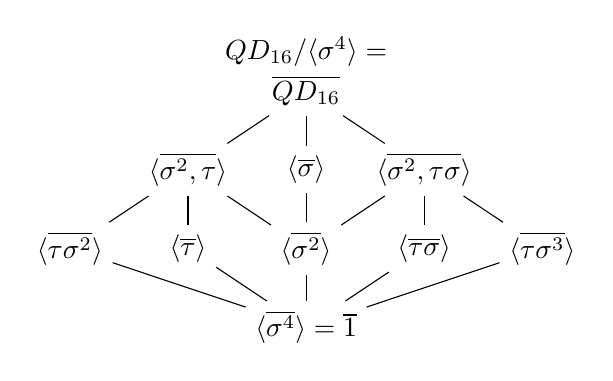
\begin{tikzpicture}
            \node at (0, 0)          (1)  {$\langle \overline{\sigma^4} \rangle = \overline{1}$};

            \node at (-3, 1)      (ts2)  {$\langle \overline{\tau \sigma^2} \rangle$};
            \node at (-1.5, 1)      (t) {$\langle \overline{\tau} \rangle$};
            \node at (0, 1)      (s2) {$\langle \overline{\sigma^2} \rangle$};
            \node at (1.5, 1)      (ts) {$\langle \overline{\tau \sigma} \rangle$};
            \node at (3, 1)      (ts3) {$\langle \overline{\tau \sigma^3} \rangle$};

            \node at (-1.5, 2)      (s2_t) {$\langle \overline{\sigma^2, \tau} \rangle$};
            \node at (0, 2)      (s) {$\langle \overline{\sigma} \rangle$};
            \node at (1.5, 2)      (s2_ts) {$\langle \overline{\sigma^2, \tau \sigma} \rangle$};
            \node at (0, 3.5)       ()  {$QD_{16}/\langle \sigma^4 \rangle =$};
            \node at (0, 3)       (QD16)  {$\overline{QD_{16}}$};
            
            \draw (1) -- (ts2);
            \draw (1) -- (t);
            \draw (1) -- (s2);
            \draw (1) -- (ts);
            \draw (1) -- (ts3);

            \draw(ts2) -- (s2_t);
            \draw(t) -- (s2_t);
            \draw(s2) -- (s2_t);
            \draw(s2) -- (s);
            \draw(s2) -- (s2_ts);
            \draw(ts) -- (s2_ts);
            \draw(ts3) -- (s2_ts);

            \draw(s2_t) -- (QD16);
            \draw(s) -- (QD16);
            \draw(s2_ts) -- (QD16);
        \end{tikzpicture}
    \end{center}

    Next, consider the generators and relations for $\overline{QD_{16}}$:
    \begin{equation*}
        \overline{QD_{16}} = \langle \overline{\sigma}, \overline{\tau} \mid \overline{\sigma}^4 = \overline{\tau}^2 = \overline{1}, \overline{\sigma \tau} = \overline{\tau \sigma^3} = \overline{\tau} \cdot \overline{\sigma}^{-1} \rangle.
    \end{equation*}
    The right-most equation among the relations: $\overline{\tau \sigma^3} = \overline{\tau} \cdot \overline{\sigma}^{-1}$ shows that the generators and relations of this quotient group are identical to those of $D_8$, mapping $s \in D_8$ to $\overline{\tau} \in \overline{QD_{16}}$ and $r \in D_8$ to $\overline{\sigma} \in \overline{QD_{16}}$. Thus we have $QD_{16}/\langle \sigma^4 \rangle \cong D_8$.
\end{proof}

\end{document}